
\renewcommand{\SS}{\mathbb{S}}
\newcommand{\Par}[2]{\mbox{$( #1, #2 )$}}
\usetikzlibrary{positioning, shapes, trees, graphs} % RNA trees
\newcommand{\scale}{0.6}

\chapter{Uvod do študia štruktúry RNA}

Na začiatku práce stručne zoznámime čitateľa s pojmamy, ktoré s RNA a jej štruktúrou súvisia.

\section{Co je RNA}

% TODO pridat nejaky vseobecny uvod, napriklad, ze RNA hraje velku ulohu pri prepise genetickej informacie a pod. potom veta ze je jednovlaknova a ze to vlakno sa sklada z molekul z 3 zloziek - cukor, fosfat a dusikata baza. Potom ze my dalej budeme na vsetko ostatne kaslat a stavebnou jednotkou bude pre nas prave baza A C G U.
Ribonukleonová kyselina, RNA, je nukleonova kyselina zlozena z nukleotidov adenin (A), uracyl (U),
cytozin (C) a guanin (G).

RNA patri medzi jednovlaknove molekuly. V snahe minimalizovat volnu energiu molekuly sa paruje sama na seba.
Vtomto hraju rolu pritazlive sily - vodikove vazby. Nukleotidy maju vzajomnu preferenciu, co znamena,
ze vazby vznikaju najcastejsie medzi bazami A - U a C - G.

Strukturu nukleovych kyselin mozeme chapat podla stupna zjednodusenia
\begin{itemize}
  \item Primarna struktura - je urcena poradim jednotlivych nukleotidov
    do polynukleotidoveho retazca
  \item Sekundarna struktura - je dana parovanim medzi bazami molekuly
  \item Terciarna struktura - priestorove usporiadanie molekuly
\end{itemize}
DNA je dvojvlaknova molekula u ktorej spojenie medzi vlaknami sa realizuje na principe
komplementarity.
Naopak, RNA je iba jednovlaknova molekula a v snahe minimalizovat volnu energiu molekuly
sa paruje sama na seba. V tomto hraju rolu pritazlive sily medzi bazami.

V praci budeme strukturou mysliet prave sekundarnu strukturu RNA, ak nebude povedane inak.

Az donedavna sa myslelo, ze funkcia RNA je obmedzena na prenos genetickej informacie z DNA
v jadre bunky do ribozomu. Napriklad pri tvorbe bielkovin (mRNA), alebo transporter aminokyselin
v ribozome bunky (tRNA).
% TODO: citacie k druhom RNA
Avsak existuje mnoho dalsich, od relativne
malych molekul tvorenych desiatkami baz, ktore pomahaju pri expresii genov
(miRNA, siRNA, tmRNA a dalsie), az po velke, tvorene tisickami nukleotidov (rRNA).

\section{Sekundarna struktura rRNA + konzervovanost}

Ako hlavny objekt zaujmu sme si spomedzi vsetkych druhov RNA vybrali prave ribozomalnu,
najma kvoli jej velkosti a tomu, ze existujucim nastrojom prave velkost robi najvacsie problemy
pri vizualizacii.

\begin{definice}[Primarna struktura RNA]
  \label{def:RNA_primarna_struktura}
  Nech $\Sigma$ je abeceda $\{A, C, G, U\}$. Potom slovo $W \in \Sigma^n$ nad touto abecedou
  je sekvencia nukleotidov (baz) RNA.
\end{definice}

Jednotlive nukleotidy sekvencie RNA budeme, ak bude jasne o co ide, oznacovat priamo poradovym
cislom, teda $i$ bude oznacovat nukleotid $W_{i}$, resp. $W[i]$.

\begin{definice}[Sekundarna struktura RNA]
  \label{def:RNA_sekundarna_struktura}
  Nech $W$ je sekvencia podla definicie \ref{def:RNA_primarna_struktura} dlzky n.
  Sekundarnou strukturou oznacime mnozinu $\SS$ parov nukleotidov \Par{i}{j} takych, ze
  pre dva pary \Par{i}{j} a \Par{k}{l} $\in \SS$ (bez ujmy na obecnosti $i \leq k$)
  plati jedno z nasledujucich:
  \begin{itemize}
    \item $i = k \iff j = l$
    \item $i < j < k < l$, cize par \Par{i}{j} predchadza par \Par{k}{l}
    \item $i < k < l < j$, cize par \Par{i}{j} obsahuje par \Par{k}{l}
  \end{itemize}
\end{definice}

%TODO: obrazok prim/sek/terc struktury RNA

Prva podmienka zabezpecuje, ze nukleotid je najviac v jednom bazickom pare, druha a tretia
hovoria o usporiadani parov, bud su na sebe nezavisle alebo na seba nadvazuju.
Posledna podmienka zakazuje existenciu pseudouzlov (pseudoknots). Pseudouzol patri medzi najcastejsie typy priestoroveho usporiadania RNA. vytvara  niekolko interakcii vramci jednej molekuly a smycky typu loops  ktore vznikaju medzi roznimy molekulami.

%TODO: pseudoknot obrazok
%TODO: 2 obrazky RNA napriec fylogenetickym stromom

\begin{figure}[H]
\centering
\includegraphics[width=140mm, height=120mm]{../img/RNA_circular_reprezentation.png}
\caption{Circular Feynman - kruhova reprezentacia sekundarnej struktury}
\label{obr:RNA_circular_representation}
\end{figure}


\subsection{Motivy}

Motivom v RNA mame na mysli casti molekuly, ktore vytvaraju urcite struktury.
Na obrazku \ref{obr:RNA_motifs} vidime motivy, ktore sa mozu v RNA vyskytovat.

Stem (stonka) je cast molekuly kde sa na seba paruju dva suvisle casti RNA vlakna.
Interior loop spaja dva stemy a medzi nimi na oboch stranach obsahuje nesparovane
bazy. Podobna je bulge (vypuklina), ale nesparovane nukleotidy ma iba z jednej strany.
Hairpin je medzi castami vlakna ktore sa paruju sami na seba.
Multibranch loop je podobna ako interior loop, ale spaja dokopy viac stemov.
V dalsom rozpravani nam bude stacit rozdelenie na stem a loop.

%TODO: ako nazyvat strukturne motivy v RNA: anglicky, alebo hladat vhodny preklad

\begin{figure}[H]
\centering
\includegraphics[width=70mm, height=70mm]{../img/struktury_v_rna.png}
\caption{Strukturalne motivy v RNA}
\label{obr:RNA_motifs}
\end{figure}

\section{Reprezentacia sekundarnej struktury}

Definicia \ref{def:RNA_sekundarna_struktura} nam ponuka reprezentovat sekundarnu strukturu
ako usporiadany strom.

\begin{figure}[H]
\centering
%TODO: vlastny obrazok... namiesto clankoveho
\includegraphics[width=130mm, height=70mm]{../img/stromova_reprezentacia_rna.png}
\caption{Varianty reprezentacie vrcholov}
\label{obr:RNA_vrcholy}
\end{figure}

\begin{definice}\label{def:strom}
  Usporiadany zakoreneny strom je orientovany graf, v ktorom plati, ze hrany su orientovane
  vzdy v smere z predka na potomka. Okrem korena ma kazdy vrchol svojho predka.
  Naviac tu existuje usporiadanie medzi potomkami.
  \\
  Usporiadany les je usporiadana mnozina stromov.
  %TODO: obrazok usporiadania stromov
\end{definice}

Bez ujmy na obecnosti budeme o RNA hovorit ako o strome, aj ked sa moze stat, ze
struktura nebude celistva (teda nieje to strom, ale les). V tom pripade ale
iba pripojime korenovy vrchol, ktoreho potomkovia budu dane stromy.

Kazdy vrchol stromu moze reprezentovat napriklad motiv v strukture RNA, nukleotid, alebo bazovy par
Priklady mozno vidiet na obrazku \ref{obr:RNA_vrcholy}.

V nasej praci vrchol stromu reprezentuje bazovy par (vnutorny vrchol) a nesparovanu bazu (list stromu).
Strukturu do ktorej patri si totiz vieme lahko zistit z potomkov vrcholu.

%rna, from 5' to 3':
% AUGCAAACUGGCACCCUCAU
% (((((...))(...))..))

\begin{center}
  \begin{minipage}{.500\textwidth}
    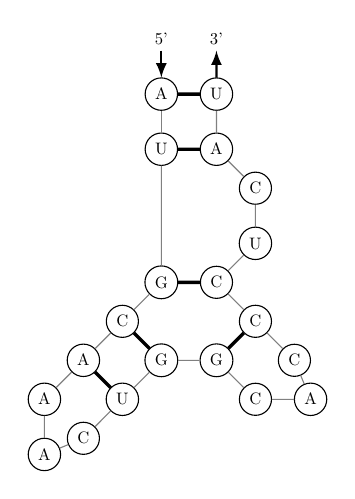
\begin{tikzpicture}[
        on grid,
        node distance = 0.7,
        -latex,
        scale = \scale,
        every node/.style = {scale = \scale},
        base/.style = {circle, draw},
        ends/.style = {draw = none, fill = none}]

      %ends, 5' a 3'
      \node[ends] (5end) {5'};
      \node[ends] (3end) [right = of 5end] {3'};

      %stem
      \node[base] (StemLeft1) [below = of 5end] {A};
      \node[base] (StemRight1) [right = of StemLeft1] {U};
      \node[base] (StemLeft2) [below = of StemLeft1] {U};
      \node[base] (StemRight2) [right = of StemLeft2] {A};

      %bulge
      \node[base] (Bulge1) [below right = of StemRight2] {C};
      \node[base] (Bulge2) [below = of Bulge1] {U};

      %stem
      \node[base] (StemRight3) [below left = of Bulge2] {C};
      \node[base] (StemLeft3) [left = of StemRight3] {G};

      %left-branch
      \node[base] (LBranchLStem1) [below left = of StemLeft3] {C};
      \node[base] (LBranchRStem1) [below right = of LBranchLStem1] {G};
      \node[base] (LBranchLStem2) [below left = of LBranchLStem1] {A};
      \node[base] (LBranchRStem2) [below left = of LBranchRStem1] {U};

      %left-branch-hairpin
      \node[base] (LBranchHairpin1) [below left = of LBranchLStem2] {A};
      \node[base] (LBranchHairpin2) [below = of LBranchHairpin1] {A};
      \node[base] (LBranchHairpin3) [below left = of LBranchRStem2] {C};

      %right-branch
      \node[base] (RBranchRStem1) [below right = of StemRight3] {C};
      \node[base] (RBranchLStem1) [below left = of RBranchRStem1] {G};

      %right-branch-hairpin
      \node[base] (RBranchHairpin1) [below right = of RBranchLStem1] {C};
      \node[base] (RBranchHairpin2) [right = of RBranchHairpin1] {A};
      \node[base] (RBranchHairpin3) [below right = of RBranchRStem1] {C};

      \begin{scope}[-]
      %pair edges
        \path[very thick]
        (StemLeft1) edge (StemRight1)
        (StemLeft2) edge (StemRight2)
        (StemLeft3) edge (StemRight3)
        (LBranchLStem1) edge (LBranchRStem1)
        (LBranchLStem2) edge (LBranchRStem2)
        (RBranchLStem1) edge (RBranchRStem1)
        ;
      %lines around molecule
        \path[color = gray]
        (StemLeft1) edge (StemLeft2)
        (StemLeft2) edge (StemLeft3)
        (StemLeft3) edge (LBranchLStem1)
        (LBranchLStem1) edge (LBranchLStem2)
        (LBranchLStem2) edge (LBranchHairpin1)
        (LBranchHairpin1) edge (LBranchHairpin2)
        (LBranchHairpin2) edge (LBranchHairpin3)
        (LBranchHairpin3) edge (LBranchRStem2)
        (LBranchRStem2) edge (LBranchRStem1)
        (LBranchRStem1) edge (RBranchLStem1)
        (RBranchLStem1) edge (RBranchHairpin1)
        (RBranchHairpin1) edge (RBranchHairpin2)
        (RBranchHairpin2) edge (RBranchHairpin3)
        (RBranchHairpin3) edge (RBranchRStem1)
        (RBranchRStem1) edge (StemRight3)
        (StemRight3) edge (Bulge2)
        (Bulge2) edge (Bulge1)
        (Bulge1) edge (StemRight2)
        (StemRight2) edge (StemRight1)
        ;
      \end{scope}

      \begin{scope}
        % edges to ends
        \path[thick]
        (5end) edge (StemLeft1)
        (StemRight1) edge (3end)
        ;
      \end{scope}
    \end{tikzpicture}
      %\caption{Molekula RNA}
      %\label{obr:RNA_rna}
  \end{minipage}
  \begin{minipage}{.450\textwidth}
    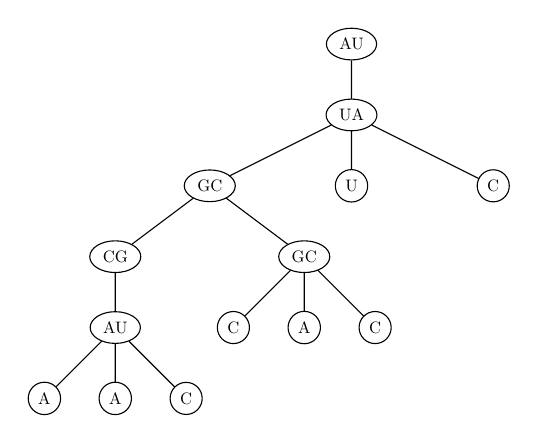
\begin{tikzpicture}[
        baseline,
        level distance = 1.5 cm,
        scale = \scale,
        every node/.style = {scale = \scale},
        basepair/.style = {ellipse, draw, minimum height = 0.3 cm, minimum width = 0.7 cm},
        unpaired/.style = {circle, draw, minimum width = 0.3 cm},
        level 2/.style = {sibling distance = 3 cm},
        level 3/.style = {sibling distance = 4 cm},
        level 4/.style = {sibling distance = 1.5 cm}
      ]
      \node[basepair] {AU}
      child {
        node[basepair] {UA}
        child {
          node[basepair] {GC}
          child {
            node[basepair] {CG}
            child {
              node[basepair] {AU}
              child {
                node[unpaired] {A}
              }
              child {
                node[unpaired] {A}
              }
              child {
                node[unpaired] {C}
              }
            }
          }
          child {
            node[basepair] {GC}
            child {
              node[unpaired] {C}
            }
            child {
              node[unpaired] {A}
            }
            child {
              node[unpaired] {C}
            }
          }
        }
        child {
          node[unpaired] {U}
        }
        child {
          node[unpaired] {C}
        }
      }
      ;
    \end{tikzpicture}
      %\caption{Stromova reprezentacia RNA}
      %\label{obr:RNA_tree}
  \end{minipage}
\end{center}




\section{RNA stromy}

%TODO grafove/stromove pojmy








%%%%%%%%%%%%%%%%%%%%%%%%%%%% TU JE SKOPIROVANA STARA CAST TOHO ISTEHO SUBORU







%\renewcommand{\SS}{\mathbb{S}}
%\newcommand{\Par}[2]{\mbox{$( #1, #2 )$}}

\chapter{Uvod do studia struktury RNA}

Na zaciatku prace strucne zoznamime citatela s pojmamy, ktore s RNA a jej strukturou suvisia.

\section{Co je RNA}

Nositelkami genetickej informacie bunky su molekuly nukleovych kyselin
tvorene retazcami nukleotidov, ktore su zakladnymi stavebnymi jednotkami
nukleovych kyselin. Vyskytuje sa niekolko variant nukleotidov (baz). U RNA su to
adein (A), guanin (G), cytozin (C), uracyl (U),
pri DNA sa namiesto uracylu vyskytuje tymin (T).
Medzi jednotlivymi bazami sa mozu vyskytovat vodikove vazby. Nukleotidy maju
vzajomnu preferenciu, co znamena, ze bazy vznikaju najcastejsie medzi A-U a C-G
u RNA a podobne A-T a C-G u DNA.
Medzi jednotlivymi bazami existuju vazby na principe komplementarity.
Vodikove vazby existuju medzi bazami A-U a C-G u RNA a podobne A-T a C-G u DNA.
Strukturu nukleovych kyselin mozeme chapat podla stupna zjednodusenia
\begin{itemize}
	\item Primarna struktura - je urcena poradim jednotlivych nukleotidov
		do polynukleotidoveho retazca
	\item Sekundarna struktura - je dana parovanim medzi bazami molekuly
	\item Terciarna struktura - 3D priestorove usporiadanie molekuly
\end{itemize}
DNA je dvojvlaknova molekula u ktorej spojenie medzi vlaknami sa realizuje na principe
komplementarity.
Naopak, RNA je iba jednovlaknova molekula a v snahe minimalizovat volnu energiu molekuly
sa paruje sama na seba. V tomto hraju rolu pritazlive sily medzi bazami.

V praci budeme strukturou mysliet prave sekundarnu strukturu RNA, ak nebude povedane inak.

Az donedavna sa myslelo, ze funkcia RNA je obmedzena na prenos genetickej informacie z DNA
v jadre bunky do ribozomu. Napriklad pri tvorbe bielkovin (mRNA), alebo transporter aminokyselin
v ribozome bunky (tRNA).
% TODO: citacie k druhom RNA
Avsak existuje mnoho dalsich, od relativne
malych molekul tvorenych desiatkami baz, ktore pomahaju pri expresii genov
(miRNA, siRNA, tmRNA a dalsie), az po velke, tvorene tisickami nukleotidov (rRNA).

\section{Sekundarna struktura rRNA + konzervovanost}

Ako hlavny objekt zaujmu sme si spomedzi vsetkych druhov RNA vybrali prave ribozomalnu,
najma kvoli jej velkosti a tomu, ze existujucim nastrojom prave velkost robi najvacsie problemy
pri vizualizacii.

\begin{definice}[Primarna struktura RNA]
  \label{def:RNA_primarna_struktura}
	Nech $\Sigma$ je abeceda $\{A, C, G, U\}$. Potom slovo $W \in \Sigma^n$ nad touto abecedou
	je sekvencia nukleotidov (baz) RNA.
\end{definice}

Jednotlive nukleotidy sekvencie RNA budeme, ak bude jasne o co ide, oznacovat priamo poradovym
cislom, teda $i$ bude oznacovat nukleotid $W_{i}$, resp. $W[i]$.

\begin{definice}[Sekundarna struktura RNA]
  \label{def:RNA_sekundarna_struktura}
	Nech $W$ je sekvencia podla definicie \ref{def:RNA_primarna_struktura} dlzky n.
	Sekundarnou strukturou oznacime mnozinu $\SS$ parov nukleotidov \Par{i}{j} takych, ze
	pre dva pary \Par{i}{j} a \Par{k}{l} $\in \SS$ (bez ujmy na obecnosti $i \leq k$)
  plati jedno z nasledujucich:
	\begin{itemize}
		\item $i = k \iff j = l$
		\item $i < j < k < l$, cize par \Par{i}{j} predchadza par \Par{k}{l}
		\item $i < k < l < j$, cize par \Par{i}{j} obsahuje par \Par{k}{l}
	\end{itemize}
\end{definice}

%TODO: obrazok prim/sek/terc struktury RNA

Prva podmienka zabezpecuje, ze nukleotid je najviac v jednom bazickom pare, druha a tretia
hovoria o usporiadani parov, bud su na sebe nezavisle alebo na seba nadvazuju.
Posledna podmienka zakazuje existenciu pseudouzlov (pseudoknots).

%TODO: pseudoknot obrazok
%TODO: 2 obrazky RNA napriec fylogenetickym stromom

\begin{figure}[H]
\centering
\includegraphics[width=140mm, height=120mm]{../img/RNA_circular_reprezentation.png}
\caption{Circular Feynman - kruhova reprezentacia sekundarnej struktury}
\label{obr:RNA_circular_representation}
\end{figure}


\subsection{Motivy}

Motivom v RNA mame na mysli casti molekuly, ktore vytvaraju urcite struktury.
Na obrazku \ref{obr:RNA_motifs} vidime motivy, ktore sa mozu v RNA vyskytovat.

Stem (stonka) je cast molekuly kde sa na seba paruju dva suvisle casti RNA vlakna.
Interior loop spaja dva stemy a medzi nimi na oboch stranach obsahuje nesparovane
bazy. Podobna je bulge (vypuklina), ale nesparovane nukleotidy ma iba z jednej strany.
Hairpin je medzi castami vlakna ktore sa paruju sami na seba.
Multibranch loop je podobna ako interior loop, ale spaja dokopy viac stemov.
V dalsom rozpravani nam bude stacit rozdelenie na stem a loop.

%TODO: ako nazyvat strukturne motivy v RNA: anglicky, alebo hladat vhodny preklad

\begin{figure}[H]
\centering
\includegraphics[width=70mm, height=70mm]{../img/struktury_v_rna.png}
\caption{Strukturalne motivy v RNA}
\label{obr:RNA_motifs}
\end{figure}










